\documentclass[a4paper,11pt]{article}
\usepackage{amsmath,amsthm,amsfonts,amssymb,amscd,amstext,vmargin,graphics,graphicx,tabularx,multicol} 
\usepackage[francais]{babel}
\usepackage[utf8]{inputenc}  
\usepackage[T1]{fontenc} 
\usepackage{pstricks-add,tikz,tkz-tab,variations}
\usepackage[autolanguage,np]{numprint} 

\setmarginsrb{1.5cm}{0.5cm}{1cm}{0.5cm}{0cm}{0cm}{0cm}{0cm} %Gauche, haut, droite, haut
\newcounter{numexo}
\newcommand{\exo}[1]{\stepcounter{numexo}\noindent{\bf Exercice~\thenumexo} : \marginpar{\hfill /#1}}
\reversemarginpar


\newcounter{enumtabi}
\newcounter{enumtaba}
\newcommand{\q}{\stepcounter{enumtabi} \theenumtabi)  }
\newcommand{\qa}{\stepcounter{enumtaba} (\alph{enumtaba}) }
\newcommand{\initq}{\setcounter{enumtabi}{0}}
\newcommand{\initqa}{\setcounter{enumtaba}{0}}

\newcommand{\be}{\begin{enumerate}}
\newcommand{\ee}{\end{enumerate}}
\newcommand{\bi}{\begin{itemize}}
\newcommand{\ei}{\end{itemize}}
\newcommand{\bp}{\begin{pspicture*}}
\newcommand{\ep}{\end{pspicture*}}
\newcommand{\bt}{\begin{tabular}}
\newcommand{\et}{\end{tabular}}
\renewcommand{\tabularxcolumn}[1]{>{\centering}m{#1}} %(colonne m{} centrée, au lieu de p par défault) 
\newcommand{\tnl}{\tabularnewline}

\newcommand{\bmul}[1]{\begin{multicols}{#1}}
\newcommand{\emul}{\end{multicols}}

\newcommand{\trait}{\noindent \rule{\linewidth}{0.2mm}}
\newcommand{\hs}[1]{\hspace{#1}}
\newcommand{\vs}[1]{\vspace{#1}}

\newcommand{\N}{\mathbb{N}}
\newcommand{\Z}{\mathbb{Z}}
\newcommand{\R}{\mathbb{R}}
\newcommand{\C}{\mathbb{C}}
\newcommand{\Dcal}{\mathcal{D}}
\newcommand{\Ccal}{\mathcal{C}}
\newcommand{\mc}{\mathcal}

\newcommand{\vect}[1]{\overrightarrow{#1}}
\newcommand{\ds}{\displaystyle}
\newcommand{\eq}{\quad \Leftrightarrow \quad}
\newcommand{\vecti}{\vec{\imath}}
\newcommand{\vectj}{\vec{\jmath}}
\newcommand{\Oij}{(O;\vec{\imath}, \vec{\jmath})}
\newcommand{\OIJ}{(O;I,J)}


\newcommand{\reponse}[1][1]{%
\multido{}{#1}{\makebox[\linewidth]{\rule[0pt]{0pt}{20pt}\dotfill}
}}

\newcommand{\titre}[5] 
% #1: titre #2: haut gauche #3: bas gauche #4: haut droite #5: bas droite
{
\noindent #2 \hfill #4 \\
#3 \hfill #5

\vspace{-1.6cm}

\begin{center}\rule{6cm}{0.5mm}\end{center}
\vspace{0.2cm}
\begin{center}{\large{\textbf{#1}}}\end{center}
\begin{center}\rule{6cm}{0.5mm}\end{center}
}



\begin{document}
\pagestyle{empty}
\titre{Contrôle : Triangles semblables}{Nom :}{Prénom :}{Classe}{Date}

\begin{flushleft}
\begin{tabular}{|m{9.5cm}|m{1.25cm}|m{1.25cm}|m{1.25cm}|m{1.25cm}|m{1.25cm}|}
\hline 
\textbf{Compétences} & \begin{center}
\textbf{N.E.}
\end{center} & \begin{center}
\textbf{M.I.}
\end{center} & \begin{center}
\textbf{M.F.}
\end{center}  & \begin{center}
\textbf{M.S.}
\end{center} & \begin{center}
\textbf{T.B.M.}
\end{center} \\ 
\hline 
Je dois savoir déterminer deux triangles semblables avec leurs côtés, angles et sommets homologues &  &  & & &\\
\hline
Je dois savoir expliquer  à l'écrit (sa démarche, son raisonnement, un calcul, un protocole de construction géométrique, un algorithme), faire une démonstration &  &  & & &\\ 
\hline


\end{tabular} 
\end{flushleft}

\textit{N.E = Non évalué ; M.I. = Maîtrise insuffisante ; M.F. = Maîtrise fragile ; M.S. = Maîtrise satisfaisante ; T.B.M. = Très bonne maîtrise}\\

\vspace*{0.5cm}

$\rightarrow$ \textit{\textbf{Dans les exercices suivants, des démonstrations sont attendues.}}\\

\vspace*{1cm}
\exo{2} Les triangles BCD et HGF sont semblables.
\begin{center}
\includegraphics[scale=1]{exossemblables.eps} 
\end{center}

\noindent \q Quel est l'homologue du sommet G ?\\
\q Quel est l'homologue du sommet C ?\\
\q Quel est l'homologue du côté [HF] ?\\
\q Quel est l'homologue de l'angle $\widehat{HGF}$ ?\\
\vspace*{1cm}

\exo{6} Dans chacun des cas suivants, prouver que les triangles sont des triangles semblables, vous pouvez utiliser la méthode que vous souhaitez.\\

\textbf{\underline{Cas 1 :}} \hspace*{8cm} \textbf{\underline{Cas 2 :}}\\

	\includegraphics[scale=1]{exosemblables1.eps} \hspace*{2cm} \includegraphics[scale=1]{exosemblables2.eps}\\
	

\newpage

\exo{3} Les triangles DEF et ACB sont des triangles semblables, calculer les longueurs DE et BC.
\begin{center}
\includegraphics[scale=0.8]{exosemblables3.eps}
\end{center}


\vspace*{1cm}

\exo{6} Pour estimer la hauteur de l'obélisque de la place de la concorde à Paris, un touriste mesurant 1,84 m regarde dans un miroir (M) dans lequel il arrive à voir le sommet S de l'obélisque. \\
Les angles $\widehat{AMT}$ et $\widehat{BMS}$ ont la même mesure.\\
\textbf{Justifier que les triangles MAT et SMB sont semblables puis calculer la hauteur SB de l'obélisque.}\\

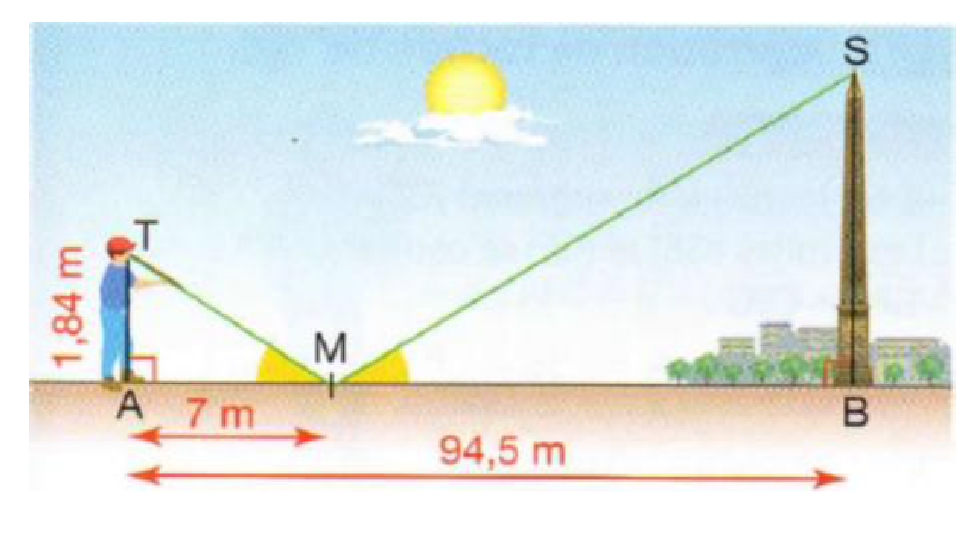
\includegraphics[scale=0.65]{interro.eps} 

\vspace*{0.75cm}

\exo{3} Sur la figure ci-dessous, les triangles BDE et BAC sont semblables.\\
\textbf{Calculer les longueurs BD et AC.}\\

\begin{center}
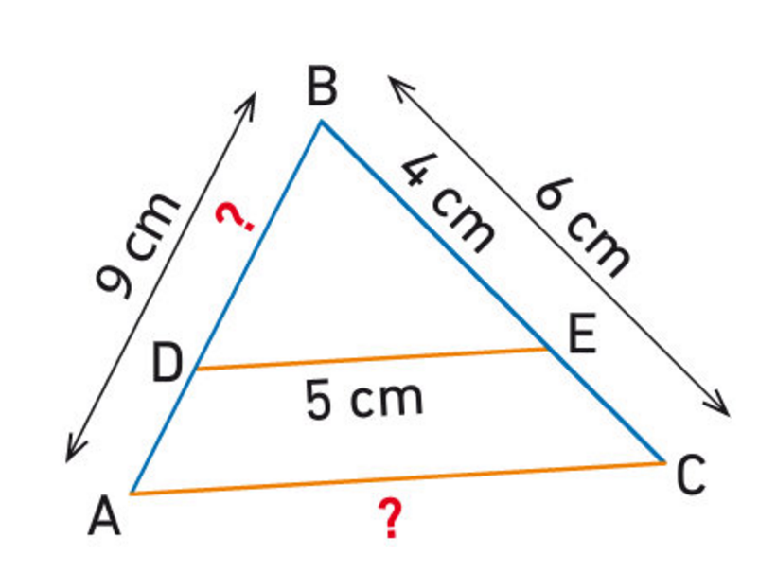
\includegraphics[scale=0.45]{thales1.eps} 
\end{center}


\end{document}
